\documentclass[a4paper, 11pt]{report}
\usepackage{blindtext}
\usepackage[T1]{fontenc}
\usepackage[utf8]{inputenc}
\usepackage{titlesec}
\usepackage{fancyhdr}
\usepackage{geometry}
\usepackage{fix-cm}
\usepackage[hidelinks]{hyperref}
\usepackage{graphicx}
\usepackage{titlesec}

\usepackage[english]{babel}

\geometry{ margin=30mm }
\counterwithin{subsection}{section}
\renewcommand\thesection{\arabic{section}.}
\renewcommand\thesubsection{\thesection\arabic{subsection}.}
\usepackage{tocloft}
\renewcommand{\cftchapleader}{\cftdotfill{\cftdotsep}}
\renewcommand{\cftsecleader}{\cftdotfill{\cftdotsep}}
\setlength{\cftsecindent}{2.2em}
\setlength{\cftsubsecindent}{4.2em}
\setlength{\cftsecnumwidth}{2em}
\setlength{\cftsubsecnumwidth}{2.5em}

\titlespacing\section{0pt}{12pt plus 4pt minus 2pt}{0pt plus 2pt minus 2pt}
\titlespacing\subsection{0pt}{12pt plus 4pt minus 2pt}{0pt plus 2pt minus 2pt}

\begin{document}
\titleformat{\section}
{\normalfont\fontsize{15}{0}\bfseries}{\thesection}{1em}{}
\titlespacing{\section}{0cm}{0.5cm}{0.15cm}
\titleformat{\subsection}
{\normalfont\fontsize{13}{0}\bfseries}{\thesubsection}{0.5em}{}
\titlespacing{\section}{0cm}{0.5cm}{0.15cm}

%=============================================================================

\pagenumbering{Alph}
\begin{titlepage}
\begin{flushright}

\includegraphics[width=4cm]{USyd}\\[2cm]
\end{flushright}
\center 
\textbf{\huge INFO1111: Computing 1A Professionalism}\\[0.75cm]
\textbf{\huge 2023 Semester 1}\\[2cm]
\textbf{\huge Self-Learning Report}\\[3cm]

\textbf{\huge Submission number: 1}\\[0.75cm]
\textbf{Github link: ??}\\[2cm]

{\large
\begin{tabular}{|p{0.35\textwidth}|p{0.55\textwidth}|}
	\hline
	{\bf Student name} & Yuri Gao\\
	{\bf Student ID} & 510015154\\
	{\bf Topic} & C \textit{Note: This must be the same as was in your topic approval}\\
	{\bf Levels already achieved} & Level A\\
	{\bf Levels in this report} & Level A\\
	\hline
\end{tabular}
}
\thispagestyle{empty}
\end{titlepage}
\pagenumbering{arabic}


%=============================================================================

\tableofcontents

%=============================================================================

\newpage
\section*{Instructions}

\textbf{Important}: This section should be removed prior to submission.

You should use this \LaTeX\ template to generate your self-learning report. Keep in mind the following key points:
\begin{itemize}
	\item \textbf{Submissions}: There will be three opportunities during the semester to submit this report. For each submission you can attempt 1 or 2 levels. Each submission should use the same report, but amended to include new information.
	\item \textbf{Assessment}: In order to achieve level B, you must first have achieved level A, and so on for each level up to level D. This means that we will not assess a higher level until a lower level has been achieved (though we will review one level higher and give you feedback to help you in refining your work).
	\item \textbf{Minimum requirement}: Remember that in order to pass the unit, you must achieve at least level A in the self-learning (unless you achieve level B in both the skills and knowledge categories).
	\item \textbf{Using this template}: When completing each section you should remove the explanation text and replace it with your material.
	\item \textbf{Referencing}: You should also ensure that any resources you use are suitably referenced, and references are included into the reference list at the end of this document. You should use the IEEE reference style \cite{usyd2} (the reference included here shows you how this can be easily achieved).
\end{itemize}


%=============================================================================


\newpage
\section{Level A: Initial Understanding}
\vspace{5mm}
\subsection{Level A Demonstration}
List the three things you will do to demonstrate your understanding of this topic.
\textit{Note: This must be the same as was in your topic approval}\\

Compilation, linking, use of libraries\\

data types and operators\\

pointers, string manipulation\\

\subsection{Learning Approach}
How did you approach your learning? Write 100 - 200 words outlining the steps you took and/or are taking to self-learn the topic you have selected.\\

During my self-teaching of C language, I first built up basic concepts and theoretical knowledge by reading classic C language tutorials and online resources. These textbooks helped me understand the basic concepts of the C language, such as the basic structure, data types, control structures, functions, and pointers. At the same time, I also referred to some high-quality online courses.\\

After establishing the basic theoretical knowledge, I started to practice and try to write some simple C language programs. I deepen my understanding of C language knowledge by solving practical problems.\\

In order to consolidate the knowledge I have learned and learn more advanced C language skills, I often communicate with my friends, share experiences, and learn from each other. At the same time, record my learning process and content to help consolidate knowledge and improve my ability to write code.\\

In short, in the process of self-learning C language, I used a variety of learning resources, combined theoretical learning and practical operation, and continuously improved my skills through discussions with friends. This comprehensive learning method has enabled me to master the C language in a relatively short period of time.\\

\subsection{Challenges and Difficulties}
What did you find most difficult? Write 100 - 200 words discussing what you have or are finding most challenging about self-learning the topic you have selected (e.g. are there any elements of the topic you have found more difficult to learn than others etc.).\\

In the process of teaching myself C language, I found that the most challenging part is to understand pointer manipulation techniques in depth. These concepts are more unique and difficult to understand than other programming basics, so I put more energy and time into research.\\

As a unique concept in C language, pointer involves address reference and memory space operation. For beginners like me, these contents may be difficult to understand. In order to master the usage of pointers, I tried to use them many times in actual programming, and gradually understood how to use pointers in dynamic memory allocation, array operations, and function parameter passing.\\

Although I encountered many challenges in the process of self-learning C language, I gradually overcome these difficulties through continuous practice, experience accumulation and interaction with others. These challenges not only gave me a deeper understanding of the underlying principles of the C language, improved my programming skills, but also inspired my enthusiasm to continue exploring other advanced technologies.\\


\subsection{Learning Sources}
Learning Source - What source did you use? (Note: Include source details such as links to websites, videos etc.).	Contribution to Learning - How did the source contribute to your learning (i.e. what did you use the source for)?

\begin{tabular}{|p{0.45\textwidth}|p{0.45\textwidth}|}
	\hline
	Learning Source - What source did you use? (Note: Include source details such as links to websites, videos etc.). & Contribution to Learning - How did the source contribute to your learning (i.e. what did you use the source for)?\\
	\hline
	https://tinyurl.com/2tkhten6 & Linking and Libraries\\
	\hline
	https://tinyurl.com/55fyfcn6 & Compilation\\
	\hline
	https://tinyurl.com/bdzj47c9 & Operators\\
	\hline
	https://tinyurl.com/3v4b26zb & Types\\
	\hline
	https://tinyurl.com/58fe7c3w & Pointers, String Manipulation\\
	\hline
\end{tabular}

\subsection{Application artifacts}
Include here a description of what you actually created (what does it do? How does it work? How did you create it?). Include any code or other related artefacts that you created (these should also be included in your github repository).

If you do include screengrabs to show what you have done then these should be annotated to explain what it is showing and what the application does.\\

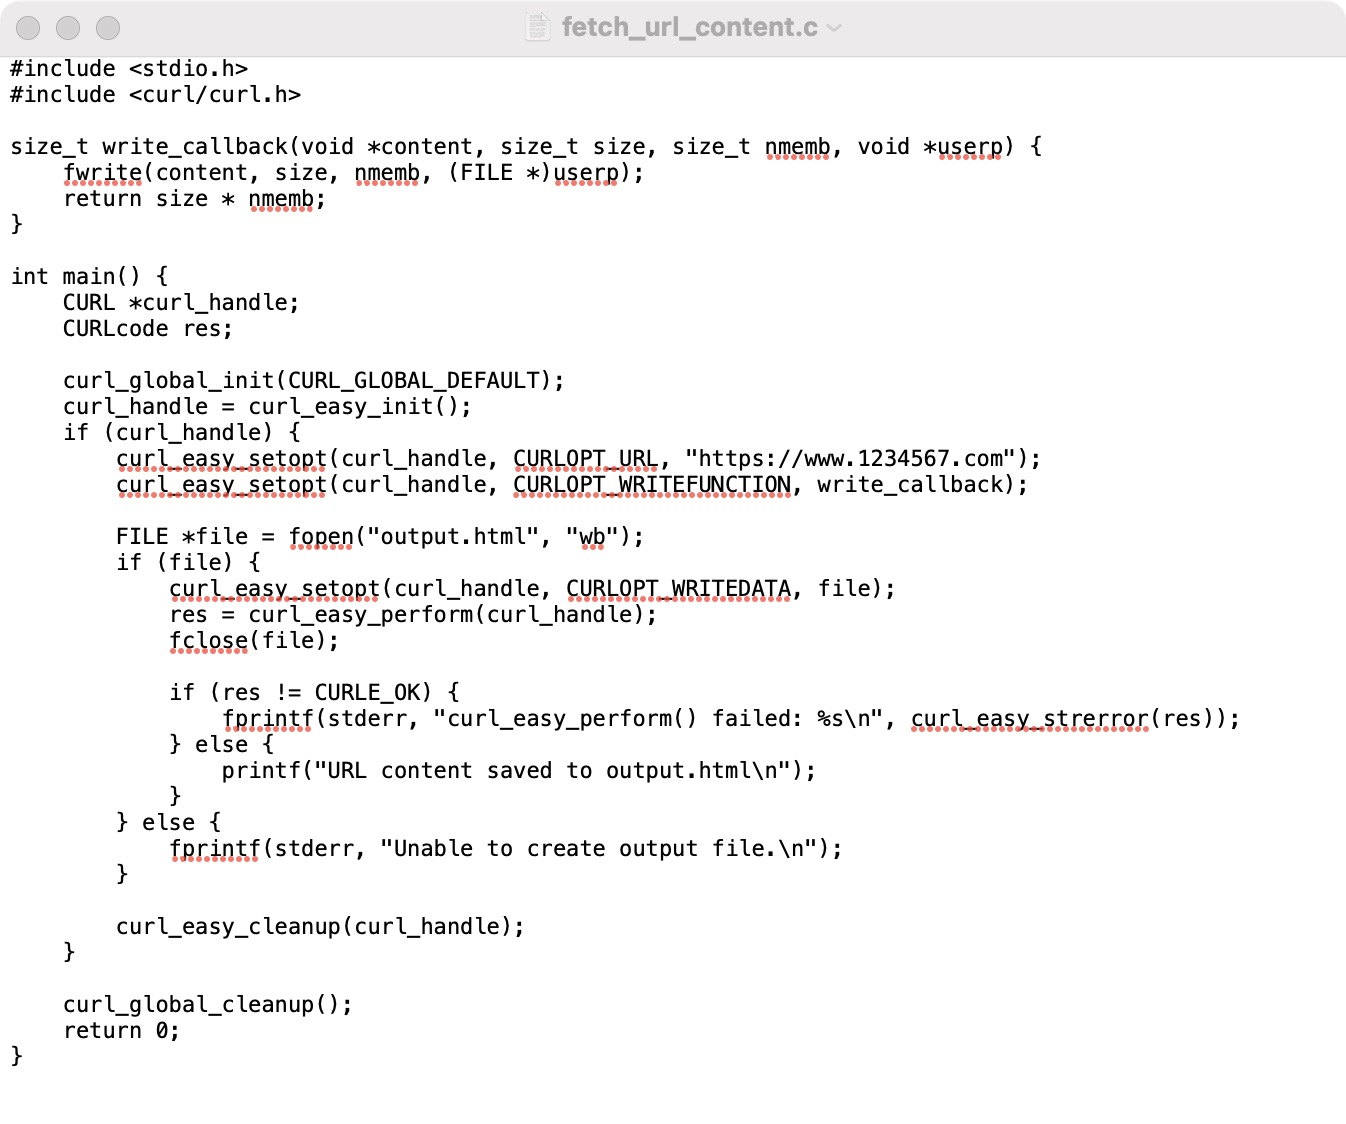
\includegraphics[width=1\linewidth]{fetch.url.content.jpeg}\\

This program uses the libcurl library to send a simple GET request to the specified URL and saves the content to a file named output.html. Next, you need to compile and link the program (you can type in the terminal: gcc -o fetch.url.content fetch.url.content.c -lcurl)\\

which will compile the fetch.url.content.c source file and link to the libcurl library. The -o option specifies the output executable file name, and the -lcurl option indicates linking to the libcurl library. After compiling, you will get an executable named fetch.url.content. You can then enter in the terminal (./fetch.url.content) \\

At this time, the program will send a GET request to https://www.1234567.com, and save the response content to the output.html file. If the request is successful, it will output "URL content saved to output.html".\\

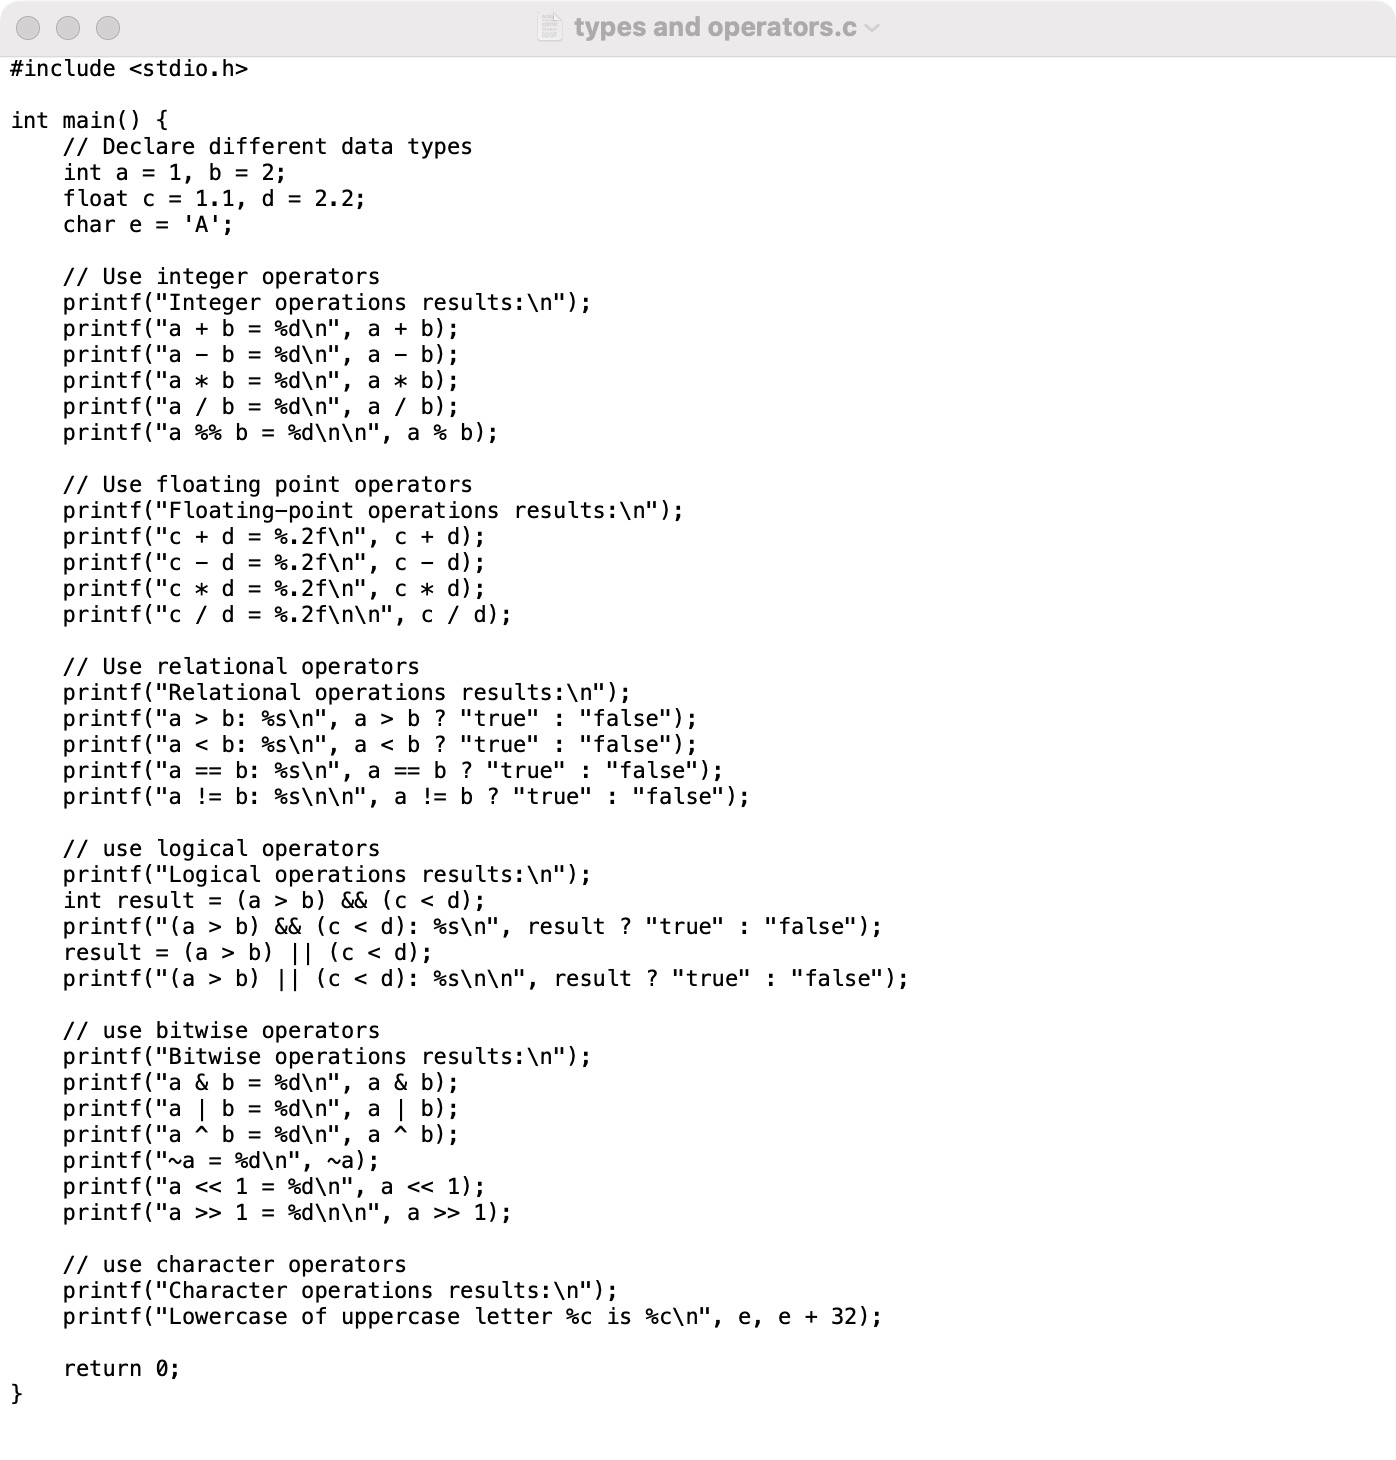
\includegraphics[width=1\linewidth]{types and operators.jpeg}\\

This program demonstrates the basic data types (integer, floating point, character) and various operators (arithmetic, relational, logical, bit, character) in C language. By running this program, that can observe the usage and results of different operators.\\

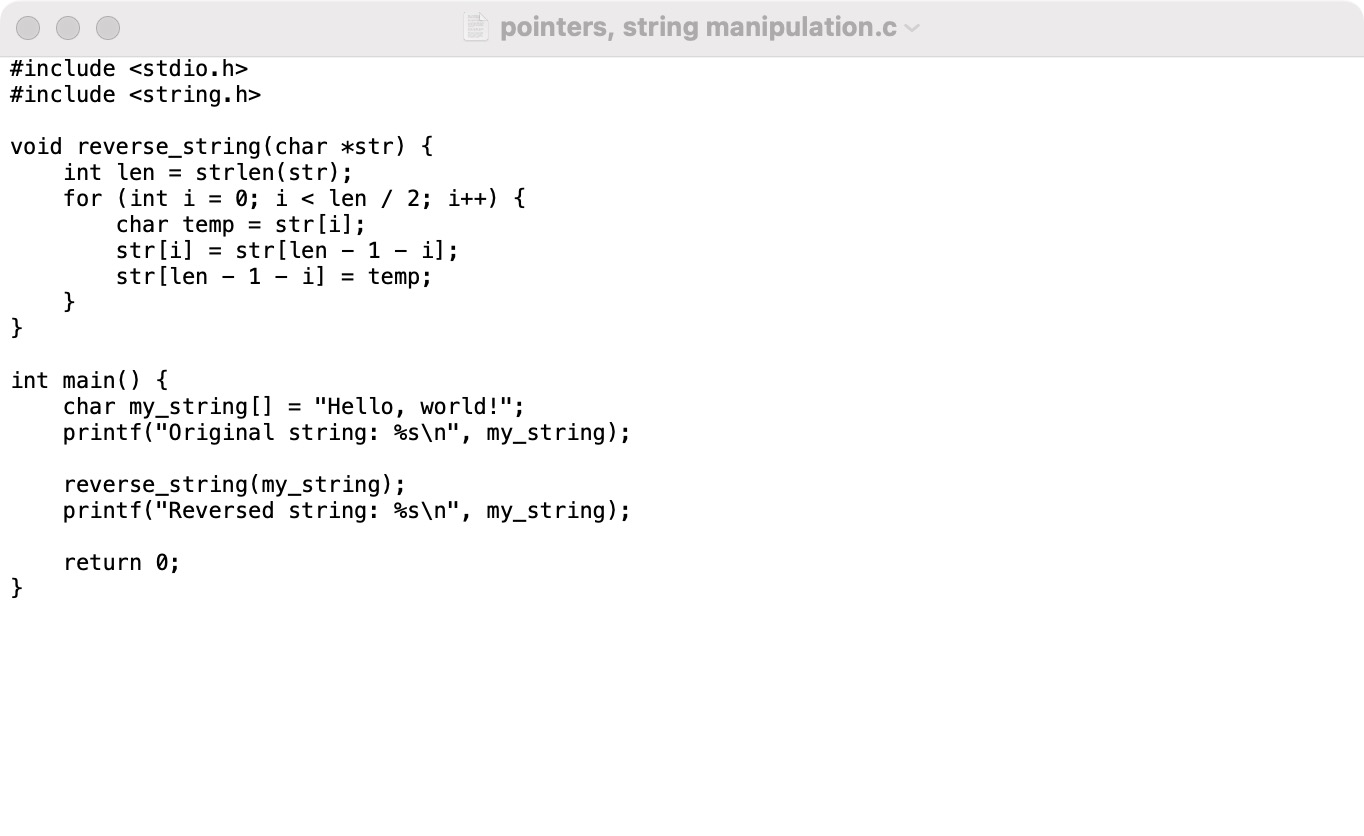
\includegraphics[width=1\linewidth]{pointers, string manipulation.jpeg}\\

This program defines a function that reverses an incoming string. We use a pointer as an argument, through which the original string is directly modified. In the main function, we create a new string and call the function defined at the beginning to reverse it. Then, we print the original string and the reversed string.\\


%=============================================================================

\newpage
\section{Level B: Basic Application}

Whilst level A is about doing something simple with the topic to just show that you have started to be able to use the tool or technology, level B is about doing something practical that might actually be useful.

\subsection{Level B Demonstration}

This is a short description of the application that you have developed in order to demonstration your understanding. (50-100 words).

\subsection{Application artifacts}

Include here a description of what you actually created (what does it do? How does it work? How did you create it?). Include any code or other related artefacts that you created (these should also be included in your github repository).

If you do include screengrabs to show what you have done then these should be annotated to explain what it is showing and what the application does.


%=============================================================================

\newpage
\section{Level C: Deeper Understanding}

Level C focuses on showing that you have actually understood the tool or technology at a relatively advanced level. You will need to compare it to alternatives, identifying key strengths and weaknesses, and the areas where this tool is most effective. 

\subsection{Strengths}
What are the key strengths of the item you have learnt? (50-100 words)

\subsection{Weaknesses}
What are the key weaknesses of the item you have learnt? (50-100 words)

\subsection{Usefulness}
Describe one scenario under which you believe the topic you have learnt could be useful. (50-100 words)

\subsection{Key Question 1}
Note: This question is in the table in the ‘Self Learning: List of Topics’ page on Canvas. (50-100 words)

\subsection{Key Question 2}
Note: This question is in the table in the ‘Self Learning: List of Topics’ page on Canvas. (50-100 words)


%=============================================================================

\newpage
\section{Level D: Evolution of skills}
\vspace{5mm}
\subsection{Level D Demonstration}

This is a short description of the application that you have developed. (50-100 words).
\textit{{\bf IMPORTANT:} You might wish to submit this as part of an earlier submission in order to obtain feedback as to whether this is likely to be acceptable for level D.}

\subsection{Application artifacts}

Include here a description of what you actually created (what does it do? How does it work? How did you create it?). Include any code or other related artefacts that you created (these should also be included in your github repository).

If you do include screengrabs to show what you have done then these should be annotated to explain what it is showing and what the application does.

\subsection{Alternative tools/technologies}
Identify 2 alternative tools/technologies that can be used instead of the one you studied for your topic. (e.g. if your topic was Python, then you might identify Java and Golang)
\subsection{Comparative Analysis}
Describe situations in which both your topic and each of the identified alternatives would be preferred over the others (100-200 words).



%=============================================================================

\newpage

\bibliographystyle{IEEEtran}
\bibliography{main}

\end{document}
\end{report}
